\documentclass[12pt]{article}
\usepackage[utf8x]{inputenc}
\usepackage{amsmath}
\usepackage{amsfonts}
\usepackage{mathrsfs}
\usepackage{natbib}
\usepackage{graphicx} % figuras
\usepackage[export]{adjustbox} % loads also graphicx
\usepackage{float}
\usepackage[font=footnotesize]{caption}
\usepackage{wrapfig}
\usepackage{authblk}
\usepackage{subfigure}
\usepackage{pifont}
\usepackage{a4wide}
%\usepackage{lipsum}
\topmargin=-2pt
\title{Name?}

\author[1]{G. B. Diaz Cortes}  
\author[1]{C. Vuik} 
\author[2]{J. D. Jansen} 
\affil[1]{Department of Applied Mathematics, TU Delft}
\affil[2]{Department of Geoscience \& Engineering, TU Delft}
\renewcommand\Authands{ and }
\date{March 2016}
\begin{document}



% Title Page




\subsection{Analysis of the snapshots}
As mentioned in the previous section, it is important to choose 'good' deflation vectors if we want to
obtain a speedup of an iterative method.\\ 
We can use solutions of a system slightly different from the original (snapshots) as deflation vectors.
For this, we need to choose the way of selecting these snapshots
wisely. The idea behind this selection is to obtain a small number of snapshots and at the same time
obtain the largest amount of information from the system.\\
In this section two lemmas are proved. The lemmas could help us to select the systems that we are going to solve for
the snapshots.\\\\
\textbf{Lemma 1.} 
Let $\mathbf{A} \in \mathbb{R}^{n\times n}$ be a non-singular matrix, such that
\begin{equation}\label{eq:ls}
\mathbf{A}\mathbf{x}=\mathbf{b},
\end{equation}
and $ \mathbf{x}_i, \mathbf{b}_i \in \mathbb{R}^{n},$ $i=1,...,m,$ where the vectors $\mathbf{b}_i$ are 
linearly independent ($l.i.$) such that: 
\begin{equation}\label{eq:lieq}
\mathbf{A}\mathbf{x}_i=\mathbf{b}_i,
\end{equation}
The following equivalence holds
\begin{equation}\label{eq:equiv}
\mathbf{x}=\sum_{i=1}^m {c}_i\mathbf{x}_i \qquad
\Leftrightarrow \qquad
\mathbf{b}=\sum_{i=1}^m {c}_i\mathbf{b}_i.
\end{equation}
Proof $\Rightarrow$
\begin{equation}\label{eq:equiv1}
\mathbf{x}=\sum_{i=1}^m {c}_i\mathbf{x}_i 
\Rightarrow 
\mathbf{b}=\sum_{i=1}^m {c}_i\mathbf{b}_i.
\end{equation}
Substituting $\mathbf{x}$ from \eqref{eq:equiv1} into $\mathbf{A}\mathbf{x}=\mathbf{b}$ leads to:
\begin{align*}
\mathbf{A}\mathbf{x}&=\sum_{i=1}^m \mathbf{A}{c}_i\mathbf{x}_i=\mathbf{A}(c_1\mathbf{x}_1+...+c_m\mathbf{x}_m).
\end{align*}
Using the linearity of $\mathbf{A}$ the equation above can be rewritten as:
\begin{align}\label{eq:bc}
\mathbf{A}c_1\mathbf{x}_1+...+\mathbf{A}c_m\mathbf{x}_m
=c_1\mathbf{b}_1+...+c_m\mathbf{b}_m=\mathbf{B}\mathbf{c}.
\end{align}
where $\mathbf{B} \in \mathbb{R}^{n\times m},$ $\mathbf{c} \in \mathbb{R}^{m}$, and the columns of $\mathbf{B}$
are the vectors $\mathbf{b}_i$.\\
From \eqref{eq:ls} and \eqref{eq:bc} we get:
\begin{align*}
\mathbf{A}\mathbf{x}=\mathbf{b}=c_1\mathbf{b}_1+...+c_m\mathbf{b}_m=\sum_{i=1}^m {c}_i\mathbf{b}_i.\\
\end{align*}
Proof $\Leftarrow $
\begin{equation}\label{eq:equiv2}
\mathbf{x}=\sum_{i=1}^m {c}_i\mathbf{x}_i\Leftarrow \mathbf{b}=\sum_{i=1}^m {c}_i\mathbf{b}_i .
\end{equation}
Substituting $\mathbf{b}$ from \eqref{eq:equiv2} into $\mathbf{A}\mathbf{x}=\mathbf{b}$ leads to:
\begin{align}\label{eq:equiv21}
\mathbf{A}\mathbf{x}&=\sum_{i=1}^m {c}_i\mathbf{b}_i.
\end{align}
Since $\mathbf{A}$ is non-singular, multiplying \eqref{eq:lieq} and \eqref{eq:equiv2} by $\mathbf{A}^{-1}$ we obtain:
\begin{align}\label{eq:equiv21}
\mathbf{x}_i&=\mathbf{A}^{-1}\mathbf{b}_i,
\end{align}
\begin{align}\label{eq:equiv21}
\mathbf{x}&=\mathbf{A}^{-1}\sum_{i=1}^m {c}_i\mathbf{b}_i=\sum_{i=1}^m {c}_i\mathbf{A}^{-1}\mathbf{b}_i=\sum_{i=1}^m {c}_i\mathbf{x}_i.
\end{align}
\begin{flushright}
$Q.E.D.$                  
\end{flushright}
\textbf{Lemma 2.}
If the the deflation matrix $\mathbf{Z}$ is constructed with a set of $m$ vectors 
\begin{equation}
 \mathbf{Z}=
\begin{bmatrix}
\mathbf{x}_1&...&...&\mathbf{x}_m
\end{bmatrix}, 
\end{equation}
such that $\mathbf{x}=\sum_{i=1}^m {c}_i\mathbf{x}_i$, with $\mathbf{x}_i$ $l.i.$, then the solution of
system $\mathbf{A}\mathbf{x}=\mathbf{b}$ is achieved within one iteration of DCG.\\
Proof.\\
The relation between $\mathbf{\hat{x}}$ and $\mathbf{x}$ is given in Equation \eqref{eq:xfromxh}:
\begin{equation*}
    \mathbf{x}=\mathbf{Q}\mathbf{b}+\mathbf{P}^T\mathbf{\hat{x}}. 
\end{equation*}
For the first term $\mathbf{Q}\mathbf{b}$, taking $\mathbf{b}=\sum_{i=1}^m {c}_i\mathbf{b}_i$ we have:

\begin{align*}
\mathbf{Q}\mathbf{b}&=\mathbf{Z}\mathbf{E}^{-1}\mathbf{Z}^T\left(\sum_{i=1}^m {c}_i\mathbf{b}_i\right)\\
&=\mathbf{Z}(\mathbf{Z}^T\mathbf{A}\mathbf{Z})^{-1}\mathbf{Z}^T\left(\sum_{i=1}^m {c}_i\mathbf{A}\mathbf{x}_i\right)\qquad \text{using Lemma 1}\\
&=\mathbf{Z}(\mathbf{Z}^T\mathbf{A}\mathbf{Z})^{-1}\mathbf{Z}^T\left( \mathbf{A}\mathbf{x}_1{c}_1+...+\mathbf{A}\mathbf{x}_m{c}_m\right) \\
&=\mathbf{Z}(\mathbf{Z}^T\mathbf{A}\mathbf{Z})^{-1}\mathbf{Z}^T(\mathbf{A}\mathbf{Z}\mathbf{c})  \\
&=\mathbf{Z}(\mathbf{Z}^T\mathbf{A}\mathbf{Z})^{-1}(\mathbf{Z}^T\mathbf{A}\mathbf{Z})\mathbf{c} \\
&=\mathbf{Z}\mathbf{c}= c_1\mathbf{x}_1+c_2\mathbf{x}_2+c_3\mathbf{x}_3+c_4\mathbf{x}_4+c_5\mathbf{x}_5\\
& =\sum_{i=1}^m {c}_i\mathbf{x}_i=\mathbf{x},
\end{align*}
\\
which is the solution of the original system.\\ 
For the second term of Equation \eqref{eq:xfromxh}, $\mathbf{P}^T\mathbf{\hat{x}}$, we compute $\mathbf{\hat{x}}$ from Equation \eqref{eq:deflsys}:
\begin{align*}
    \mathbf{P}\mathbf{A}\hat{\mathbf{x}}&=\mathbf{P}\mathbf{b}\\
    \mathbf{A}\mathbf{P}^T\hat{\mathbf{x}}&=(\mathbf{I}-\mathbf{A}\mathbf{Q})\mathbf{b} \qquad \text{using \ref{defprop} f) and definition of $\mathbf{P}$,}\\
        \mathbf{A}\mathbf{P}^T\hat{\mathbf{x}}&=\mathbf{b}-\mathbf{A}\mathbf{Q}\mathbf{b}\\
        \mathbf{A}\mathbf{P}^T\hat{\mathbf{x}}&=\mathbf{b}-\mathbf{A}\mathbf{x}=0 \qquad \text{taking $\mathbf{Q}\mathbf{b}=\mathbf{x}$ from above,}\\
          \mathbf{P}^T\hat{\mathbf{x}}&=0 \qquad \text{as $\mathbf{A}$ is invertible.}
\end{align*}
Then we have achieve the solution $\mathbf{x}$ in one step of DICCG.\\


\subsubsection{Accuracy of the snapshots.}\label{accs}

If we use an iterative method to obtain an approximate solution $\mathbf{x}^k$, for the system $\mathbf{A}\mathbf{x}=\mathbf{b},$ we cannot compute the relative error of the approximation with respect to the true solution, 
$$\frac{||\mathbf{x}-\mathbf{x}^k||_2}{||\mathbf{x}||_2}.$$
Instead, we compute the relative residual, $$ \frac{||\mathbf{r}^k||_2}{||\mathbf{b}||_2}\leq \epsilon,$$
and we set a stopping criterium $\epsilon$ or tolerance, that is related to the relative error as follows (see Appendix \ref{a2}),
$$\frac{||\mathbf{x}-\mathbf{x}^k||_2}{||\mathbf{x}||_2}\leq \kappa_2(\mathbf{A}) \epsilon=\varepsilon,$$
where $\kappa_2(\mathbf{A})$ is the condition number of the matrix $\mathbf{A}$\\
Diverse tolerance values can be used in the experiments for the snapshots as well as for the solution of the original system. \\
If the maximum residual for the snapshots is $\epsilon=10^{-\eta}$ then the error of the snapshots is given by
$$\frac{||\mathbf{x}_i-\mathbf{x}_i^k||_2}{||\mathbf{x}_i||_2}\leq \kappa_2(\mathbf{A})\times 10^{-\eta}=\varepsilon.$$
If we use $m$ snapshots obtained with an iterative method to compute the solution of $\mathbf{x}$, after one iteration of DCG we obtain
$$\hat{x}=\sum_{i=1}^m {c}_i\mathbf{x}_i^{k(i)}.$$
The error of this solution is given by:
$$\frac{||\mathbf{x}-\mathbf{x}^k||_2}{||\mathbf{x}||_2}=
\frac{||\sum_{i=1}^m {c}_i(\mathbf{x}_i-\mathbf{x}_i^{k})||_2}{||\sum_{i=1}^m {c}_i\mathbf{x}_i||_2}\leq
\frac{\sum_{i=1}^m| {c}_i|\times \kappa_2(\mathbf{A})\times 10^{-\eta}}{||\sum_{i=1}^m {c}_i\mathbf{x}_i||_2}.
$$
Which means that the approximation has an error of $\mathcal{O}(\kappa_2\times10^{-\eta}).$
\\From Lemma 2 we know that if we use the snapshots $\mathbf{x}_i$ as deflation vectors, for the deflation method $$\mathbf{Q}\mathbf{b}=\mathbf{x}.$$ 
If the approximation has an error $\mathcal{O}(\kappa_2\times10^{-\eta})$, then the solution achieved with deflation will have the same error, 
$$\mathbf{Q}\mathbf{b}=\mathbf{x}^k+\mathcal{O}(\kappa_2\times10^{-\eta}).$$
Therefore, is important to take into account the condition number of the matrix related to the system  and the accuracy of the deflation vectors.
\subsubsection{Boundary conditions.}
From Lemma 2, we know that if we use as deflation vectors a set of $m$ snapshots $$\mathbf{Z}=[\mathbf{x}_1\qquad ...\qquad \mathbf{x}_m],$$ such that $\mathbf{x}=\sum_{i=1}^m {c}_i\mathbf{x}_i$, where $\mathbf{x}$ is the solution of the system $\mathbf{A}\mathbf{x}=\mathbf{b}$, the solution of the latter system is achieved within one iteration of DICCG. \\
In our application, only a small number ($m$) of elements of the right hand side vector ($\mathbf{b}$)
are changed for various situations. This implies that every $\mathbf{b}$ can be written as $\mathbf{b}=\sum_{i=1}^m {c}_i\mathbf{b}_i.$ Using Lemma 1, this implies that $\mathbf{x}$ is such that 
$\mathbf{x}\in span\{ \mathbf{x}_1, ...,  \mathbf{x}_m\}$, which is called the solution span.
Therefore, it is necessary to find the solution span of the system, such that the sum of the elements in the solution span and the sum of right hand sides give as result the original system. In this section we explore the subsystems that should be chosen, depending on the boundary conditions of the original system. 
\subsubsection*{{Neumann Boundary conditions}}
When we have Neumann boundary conditions everywhere, the resulting matrix $\mathbf{A}$ is singular, and
$\mathbf{A}[1\quad 1\quad ...\quad 1\quad 1]^T=\mathbf{0},$ $Ker(\mathbf{A})=span([1\quad 1\quad ...\quad 1\quad 1]^T)$. 
Note that $\mathbf{A}\mathbf{x}=\mathbf{b}$ has only a solution if $\mathbf{b}\in span\{\mathbf{a}_1,...,\mathbf{a}_n\}$ (with $\mathbf{a}_i$ the $i-th$ column of $\mathbf{A}$), which is equivalent to $\mathbf{b}\perp Ker(\mathbf{A}) $ \cite{Strang09}.
This implies that if we have $m$ sources with value ${s}_i$ for the vector $\mathbf{b}_i$, we need that 
$$\sum_{j=1}^ m {s}^{j}_i=0.$$
Then, for each nonzero  right hand side we need to have at least two sources. Therefore, we can have at most $m-1$ linearly independent right hand sides $\mathbf{b}_{i}$ containing two sources.\\
This means that the solution space has dimention $m-1$ and it can be spanned by $ span\{\mathbf{x}_1,...,\mathbf{x}_{m-1}\}$.
Each of this subsystems will have the same no-flux conditions (Neumann) in all the boundaries.
As the original system is a linear combination of the subsystems (Lemma 1), the deflation vectors can be chosen as the solutions corresponding to the subsystems. Therefore, the deflation matrix will be given by:
$$\mathbf{Z}=[\mathbf{x}_1\qquad ...\qquad \mathbf{x}_m],$$
and if the accuracy of the snapshots used as deflation vectors is good enough (see Section \ref{accs}), the solution is expected to be achieved within one iteration. 
\subsubsection*{{Dirichlet Boundary conditions}}
In this case, the right hand side of the system can contain the values of the boundary $\mathbf{b}_b$ and the sources of the system $\mathbf{s}_i$. 
If we have $m$ sources, as in the previous case, the right hand side will be given by:
$$\mathbf{b}=\sum_{i=1}^{m-1} {c}_i\mathbf{s}_i+\mathbf{b}_b.$$
The subsystems will be $m+1$, where one of them corresponds to the boundary conditions
 $\mathbf{A}\mathbf{x}_b=\mathbf{b}_b,$
 and the other $m-1$ will correspond to the sources
$\mathbf{A}\mathbf{x}_i=\mathbf{s}_i.$
Therefore, one of the snapshots will be the system with no sources and the Dirichlet boundary conditions of the original system. And the other $m$ snapshots will correspond to the $m$ sources with homogeneous Dirichlet boundary conditions. Then, the solution space will be given by $ span\{\mathbf{x}_1,...,\mathbf{x}_{m-1},\mathbf{x}_b\}$
If we use the solution of the $m$ snapshots as deflation vectors, if the accuracy is enough, we will obtain the solution within one iteration.

\subsection*{Flow through porous media}

\hspace{0.5cm}To describe single-phase flow through a porous medium, we use the continuity equations:
\begin{equation}\label{eq:ce}
\frac{\partial (\rho \phi)}{\partial t}+ \nabla \cdot ( \rho \mathbf{v})=q, \qquad \mathbf{v}=-\frac{\mathbf{K}}{\mu}(\nabla \mathbf{p}-\rho g\nabla z),
\end{equation}
or
\begin{equation}\label{eq:ce1}
\frac{\partial (\rho \phi)}{\partial t}- \nabla \cdot \left( \frac{\rho\mathbf{K}}{\mu}(\nabla \mathbf{p}-\rho g\nabla z)\right)=q.
\end{equation}
Where the primary unknown is the pressure $\mathbf{p}$.  The fluid  $\rho=\rho(\mathbf{p})$ and rock $\phi=\phi(\mathbf{p})$ compressibilities can be pressure dependent.
Rock compressibility is defined by:
\begin{equation*}
 c_r=\frac{1}{\phi}\frac{d\phi}{dp}=\frac{ln(\phi)}{dp},
\end{equation*}
If the rock compressibility is constant, the previous equation can be integrated as:
\begin{equation*}
 \phi(p)=\phi_0 e^{c_r(p-p_0)}.
\end{equation*}
Fluid compressibility is defined as:
\begin{equation}\label{eq:fc}
 c_f=\frac{1}{\rho}\frac{d\rho}{dp}=\frac{ln(\rho)}{dp}.
\end{equation}
If the fluid compressibility is constant, the previous equation can be integrated as:
\begin{equation}\label{eq:rhoeq}
 \rho(\mathbf{p})=\rho_0 e^{c_f(\mathbf{p}-\mathbf{p}_0)}.
\end{equation}

Using implicit discretization, Equation \eqref{eq:ce} becomes:
\begin{equation}\label{eq:ce2}
 \frac{(\mathbf{\phi}\mathbf{\rho})^{n+1}-(\mathbf{\phi}\mathbf{\rho})^{n}}{\Delta t^n}
 +\nabla \cdot (\mathbf{\rho} \mathbf{v})^{n+1}=\mathbf{q}^{n},
\qquad
\mathbf{v}^{n+1}= -\frac{\mathbf{K}}{\mu^{n+1}}[\nabla(\mathbf{p}^{n+1})-g\mathbf{\rho}^{n+1}\nabla(\mathbf{z})].
\end{equation}
If $\mathbf{\phi}$ and $\mathbf{\rho}$ depend nonlinearly on $\mathbf{p}$ we have a nonlinear system 
of equations to be solved for each time step.  \\
Assuming no gravity terms, Equation \eqref{eq:ce2}
can be rewritten as:
\begin{equation}\label{eq:ce3}
 \frac{\mathbf{\phi}(\mathbf{p}^{n+1})\mathbf{\rho}(\mathbf{p}^{n+1})
 -\mathbf{\phi}(\mathbf{p}^{n})\mathbf{\rho}(\mathbf{p}^{n})}{\Delta t^n}
 +\nabla \cdot (\mathbf{\rho} \mathbf{v})^{n+1}=\mathbf{q}^{n},
\qquad
\mathbf{v}^{n+1}= -\frac{\mathbf{K}}{\mu^{n+1}}\nabla(\mathbf{p}^{n+1}).
\end{equation}
Or:
\begin{equation}\label{eq:ce4}
 \frac{\mathbf{\phi}(\mathbf{p}^{n+1})\mathbf{\rho}(\mathbf{p}^{n+1})
 -\mathbf{\phi}(\mathbf{p}^{n})\mathbf{\rho}(\mathbf{p}^{n})}{\Delta t^n}
 -\nabla \cdot (\mathbf{\rho}(\mathbf{p}^{n+1}) 
 \frac{\mathbf{K}}{\mu^{n+1}}\nabla(\mathbf{p}^{n+1}))-\mathbf{q}^{n}=0.
\end{equation}
The latter system can be written in short vector form as:
\begin{equation}\label{NR}
 \mathbf{F}(\mathbf{p}^{n+1};\mathbf{p}^n)=0,
\end{equation}
with $\mathbf{p}^n$ the vector of unknown state variables at the time step $n$.\\
This non-linear system can be solved by Newton Rhapson (NR) method, the $(i+1)$-th iteration approximation is obtained from:
$$\frac{\partial \mathbf{F}(\mathbf{x}^i)}{\partial \mathbf{x}^i}\delta\mathbf{x}^i=-\mathbf{F}(\mathbf{x}^i),
\qquad \mathbf{x}^{i+1}=\mathbf{x}^i+\delta \mathbf{x}^{i+1},$$
where $\mathbf{J}(\mathbf{x}^i)=\frac{\partial \mathbf{F}(\mathbf{x}^i)}{\partial \mathbf{x}^i}$ is the 
Jacobian matrix, and $\delta \mathbf{x}^{i+1}$ is the NR update at iteration step $i+1$.\\
Well model\\
In reservoirs, wells are typically drilled to extract or inject fluids. If the injection or production rates are known it is necessary to know the well pressure. Meanwhile, if the well pressure is known, the objective will be to compute the flow rate in or out of the reservoir. Fluids are injected into a well at constant surface rate or constant bottom-hole pressure, and are produced at constant bottom-hole pressure or a constant surface rate.\\
Close to a well, the pressure presents nonlinear gradients in the radial direction. In reservoir simulation, it is possible to capture this effect with a very fine grid. It is also possible to use models that take into account an additional pressure drop based on analytical or semi-analytical solutions for the flow around the well. A widely used model is Peacemans's model, that takes into account the above-mentioned pressure drop. 
This model is a linear relationship between the bottom-hole pressure and the surface flow rate in a well:
$$q_0=J(p_R-p_{bhp}),$$
where $J$ is the productivity or injectivity index.\\




\newpage
\subsection*{Compressible Problem}

\begin{wrapfigure}{R}{5cm}
\centering 
\vspace{-10pt}
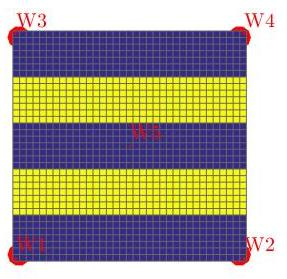
\includegraphics[width=4.5cm,height=4.5cm,keepaspectratio]{perm_comp.jpg}
 \vspace{-5pt}
\caption{ Heterogeneous permeability, 5 wells, compressible problem.}\label{fig:pc}
\vspace{-15pt}
\end{wrapfigure} 

A grid of $35\times 35$ cells is used with Newmann boundary conditions only. The domain consists of layers with two different permeability values (see Figure \ref{fig:pc}). The first layer has a permeability of $\sigma_1 = 30mD$, and the permeability of the second layer is $\sigma_2 = 3mD$. Therefore the permeability contrast between the layers is $10^{-1}$.The initial pressure of the reservoir is set as 200 bars. Four wells are positioned in the corners of the domain with a bhp of 100 bars, and a well is placed in the center of the domain with a bhp of 600 bars.
 For the first set of problems, we use the solution of the first 10 time steps with the same configuration as the problem as deflation vectors. We solve the rest of the time steps with DICCG$_{10}$ method with the 10 snapshots as deflation vectors and with 5 basis POD vectors as deflation vectors, DICCG$_{POD}$.
 For the second set of experiments, we use the same configuration as in the original problem but we vary the configuration of the wells. One corner well has the same pressure as the reservoir (200 bar), the other corner wells have a pressure of 100 bars and the central well has a pressure of 500 bars. 

\begin{itemize}
\begin{minipage}{.6\textwidth}
\item[]  $System$ $configuration$
\item[] Initial pressure 200 bar.
 \item[]  W1 =  W2 = W3 = W4 = 100 bar.
 \item[] W5 = 600 bars.\\
 \end{minipage}%
\begin{minipage}{.4\textwidth}
\item[] $Boundary$ $conditions:$\\
\item[] $\frac{\partial P(y=1)}{\partial n}=\frac{\partial P(y=ny)}{\partial n}=$
\item[] $\frac{\partial P(x=1)}{\partial n}=\frac{\partial P(x=nx)}{\partial n}=0$.
\end{minipage}
\begin{minipage}{.8\textwidth}
\item[] $Snapshots (second set of experiments)$ 
 \item[] $\mathbf{z}_1$:  W2 = W3 = W4 =  100 bars, 
 W1 = 200 bars, W5 = 500 bars.
\item[] $\mathbf{z}_2$: W1 = W3 = W4 = 100 bars,
 W2 = 200 bars, W5 = 500 bars.
\item[] $\mathbf{z}_3$: W1 = W2 = W4 = 100 bars,
 W3 = 200 bars, W5 =  500 bars.
\item[] $\mathbf{z}_4$:  W1 = W2 = W3 = 100 bars,
 W4 = 200 bars, W5 =  500 bars.\\
\end{minipage}%
\end{itemize}
The simulation was performed during 152 days with 52 time steps and a time step of 3 days. The tolerance of the NR method and the linear solvers was of $10^{-5}$.\\
\emph{\textbf{Case 1}}\\
In Figure \ref{fig:compsol}, the solution obtained with ICCG method is presented, the solution is the same for all methods. The upper left figure represents the pressure field at the final time step. The upper right figure represents the pressure across the diagonal joining the (0,0) and (35,35) grid cells. We observe the initial pressure (200 bars) in this diagonal and the evolution of the pressure field through the time. In the lower figure we observe the surface volume rate for the five wells during the simulation.\\
\begin{figure}[!h]
\centering
\begin{minipage}{.7\textwidth}
 \centering
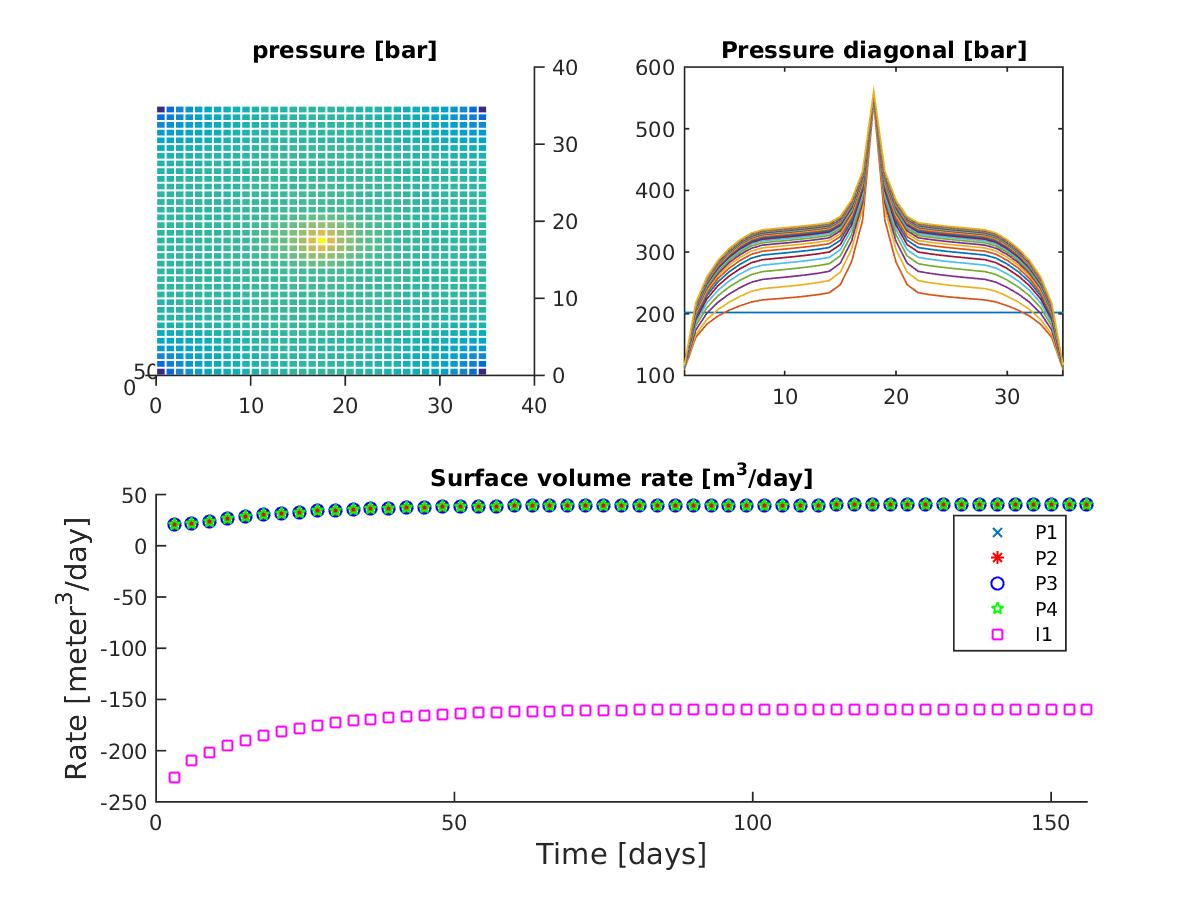
\includegraphics[width=10cm,height=10cm,keepaspectratio]
{solutionIC.jpg}
\caption{Solution of the compressible problem solved with the ICCG method.}
\label{fig:compsol}
\end{minipage}
\end{figure}

\begin{figure}[!h]
\centering
\begin{minipage}{.6\textwidth}
 \centering
\includegraphics[width=6.5cm,height=6.5cm,keepaspectratio]
{/dev/media/Sphinx/Doctorado_Delft/Results/16_08/22/size_35perm_1_5wells_c_1e-3/eigs/eigs1stepA.jpg}
\caption{Eigenvalues of the matrix, time step 1.}
\label{fig:eigs_A}
\end{minipage}
\end{figure}
The number of iterations necessary to reach convergence with the linear solvers is presented for the first four NR iterations in Figure \ref{fig:NR_IC} for the ICCG method, Figure \ref{fig:NR_D10} for the deflated method DICCG$_{10}$ using 10 snapshots as deflation vectors, Figure \ref{fig:NR_POD1_5} DICCG$_{PODi}$ using the first 5 basis vectors of POD as deflation vectors and Figure \ref{fig:NR_POD6_10} DICCG$_{PODf}$ using the last 5 basis vectors of POD as deflation vectors. 
The eigenvalues of the matrices are presented in Figure \ref{fig:eigs_A} for the original system matrix $\mathbf{J}$ for the first timestep, Figure \ref{fig:eigs_MA} the preconditioned system, Figure \ref{fig:eigs_MA} the deflated system $DICCG_{10}$, Figure \ref{fig:eigs_POD1_5} the deflated system combined with POD $DICCG_{PODi}$ using the eigenvectors corresponding to the first five larges eigenvalues and Figure \ref{fig:eigs_POD1_5} the deflated system combined with POD $DICCG_{PODf}$ for the last five eigenvalues. The eigenvalues of the snapshot correlation matrix $\mathbf{R}=\frac{1}{m}\mathbf{Z}\mathbf{Z}^T$ are presented in Figure \ref{fig:eig_POD}. 
%The eigenvalues of the covariance matrix  $\bar{\mathbf{R}}=\frac{1}{m}\sum_{i=1}^{m}(\mathbf{z}_i-\mathbf{z})(\mathbf{z}_i-\mathbf{z})^T$ are presented in Figure \ref{fig:eig_PODr}.\\

\begin{figure}[!h]
\centering
\begin{minipage}{.4\textwidth}
 \centering
\includegraphics[width=6.5cm,height=6.5cm,keepaspectratio]
{/dev/media/Sphinx/Doctorado_Delft/Results/16_08/22/size_35perm_1_5wells_c_1e-3/iterations_4NR.jpg}
\caption{Number of iterations of the ICCG method for the first four NR iterations.}
\label{fig:NR_IC}
\end{minipage}%
\hspace{15mm}
\begin{minipage}{.4\textwidth}
 \centering
 \vspace{-5mm}
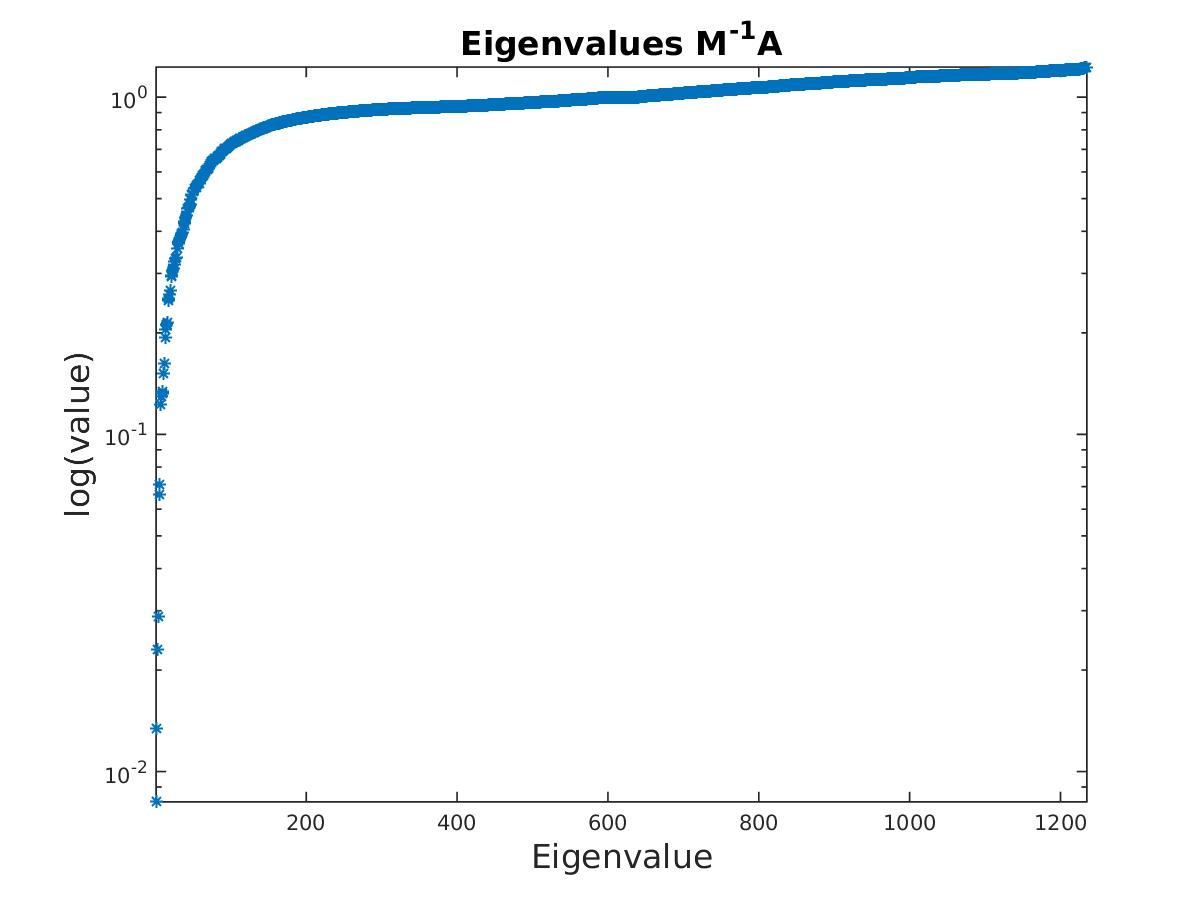
\includegraphics[width=6.5cm,height=6.5cm,keepaspectratio]
{/dev/media/Sphinx/Doctorado_Delft/Results/16_08/22/size_35perm_1_5wells_c_1e-3/eigs/eigs1step.jpg}
\caption{Eigenvalues of the preconditioned matrix, time step 1.}
\label{fig:eigs_MA}
\end{minipage}
\end{figure}

\begin{figure}[!h]
\centering
\begin{minipage}{.4\textwidth}
 \centering
\includegraphics[width=6.5cm,height=6.5cm,keepaspectratio]
{/dev/media/Sphinx/Doctorado_Delft/Results/16_08/22/size_35perm_1_5wells_c_1e-3dv_10/iterations_4NR.jpg}
\caption{Number of iterations of the DICCG$_{10}$ method for the first four NR iterations.}
\label{fig:NR_D10}
\end{minipage}%
\hspace{15mm}
\begin{minipage}{.4\textwidth}
 \centering
\includegraphics[width=6.5cm,height=6.5cm,keepaspectratio]
{/dev/media/Sphinx/Doctorado_Delft/Results/16_08/22/size_35perm_1_5wells_c_1e-3dv_10/eigs/eigsPA11step.jpg}
\caption{Eigenvalues of the deflated system DICCG$_{10}$ with 10 deflation vectors.}
\label{fig:eigs_PA}
\end{minipage}
\end{figure}


\begin{figure}[!h]
\centering
\begin{minipage}{.4\textwidth}
 \centering
\includegraphics[width=6.5cm,height=6.5cm,keepaspectratio]
{/dev/media/Sphinx/Doctorado_Delft/Results/16_08/22/size_35perm_1_5wells_c_1e-3dv_10pod12345/eig_pod.jpg}
\caption{Eigenvalues of the snapshot correlation matrix $\mathbf{R}=\frac{1}{m}\mathbf{Z}\mathbf{Z}^T$.}
\label{fig:eig_POD}
\end{minipage}
\end{figure}


\begin{figure}[!h]
\centering
\begin{minipage}{.4\textwidth}
 \centering
\includegraphics[width=6.5cm,height=6.5cm,keepaspectratio]
{/dev/media/Sphinx/Doctorado_Delft/Results/16_08/22/size_35perm_1_5wells_c_1e-3dv_10pod12345/iterations_4NR.jpg}
\caption{Number of iterations of the DICCG$_{POD}$ method for the first four NR iterations, eigenvectors [1-5].}
\label{fig:NR_POD1_5}
\end{minipage}%
\hspace{15mm}
\begin{minipage}{.4\textwidth}
 \centering
\includegraphics[width=6.5cm,height=6.5cm,keepaspectratio]
{/dev/media/Sphinx/Doctorado_Delft/Results/16_08/22/size_35perm_1_5wells_c_1e-3dv_10pod12345/eigs/eigsPA11step.jpg}
\caption{Eigenvalues of the deflated system DICCG$_{POD}$ with 10 deflation vectors, eigenvectors [1-5].}
\label{fig:eigs_POD1_5}
\end{minipage}
\end{figure}
\begin{figure}[!h]
\centering
\begin{minipage}{.4\textwidth}
 \centering
\includegraphics[width=6.5cm,height=6.5cm,keepaspectratio]
{/dev/media/Sphinx/Doctorado_Delft/Results/16_08/22/size_35perm_1_5wells_c_1e-3dv_10pod678910/iterations_4NR.jpg}
\caption{Number of iterations of the DICCG$_{POD}$ method for the first four NR iterations, eigenvectors [6-10].}
\label{fig:NR_POD6_10}
\end{minipage}%
\hspace{15mm}
\begin{minipage}{.4\textwidth}
 \centering
\includegraphics[width=6.5cm,height=6.5cm,keepaspectratio]
{/dev/media/Sphinx/Doctorado_Delft/Results/16_08/22/size_35perm_1_5wells_c_1e-3dv_10pod678910/eigs/eigsPA11step.jpg}
\caption{Eigenvalues of the deflated system DICCG$_{POD}$ with 10 deflation vectors, eigenvectors [6-10].}
\label{fig:eigs_POD6_10}
\end{minipage}
\end{figure}
We observe that the number of iterations for the first and second NR iterations is lower for the deflated methods compared with the ICCG method. However, we observe that the time step when convergence is achieved for the NR cycle is larger for these methods with respect to the ICCG method. We also observe that for the first NR iteration, the decrease is larger for the deflated method with 10 snapshots as deflation vectors.\\
\newpage
\emph{\textbf{Case 2}}\\
In the second case, we compute the first 4 time steps varying the bhp of the wells, as described above. Figure \ref{fig:compsolvw} presents the solution obtained with ICCG method is presented. The upper left figure represents the pressure field at the final time step. The upper right figure represents the pressure across the diagonal joining the (0,0) and (35,35) grid cells. We can observe the initial pressure (200 bars) in this diagonal and the evolution of the pressure field through the time. In the lower figure, we observe the surface volume rate for the five wells during the simulation.

\begin{figure}[!h]
\centering
\begin{minipage}{.7\textwidth}
 \centering
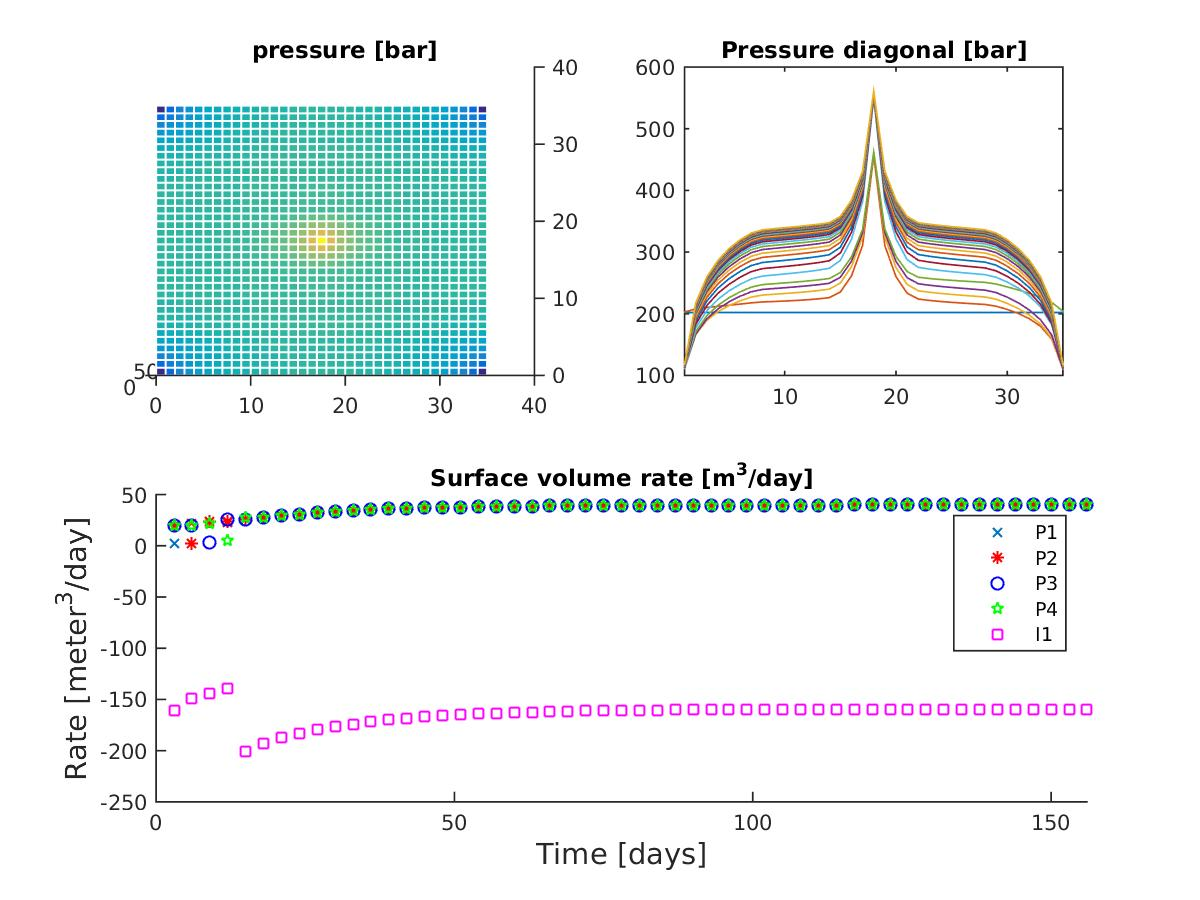
\includegraphics[width=10cm,height=10cm,keepaspectratio]
{solutionvw_IC.jpg}
\caption{Solution of the compressible problem solved with the ICCG method, varying the bhp of the first 4 time steps.}
\label{fig:compsolvw}
\end{minipage}
\end{figure}
The number of iterations necessary to achieve convergence with the linear solvers for this second problem is presented for the first four NR iterations in Figure \ref{fig:vwNR_IC} for the ICCG method, Figure \ref{fig:vwNR_D10} for the deflated method DICCG$_{10}$ using 10 snapshots as deflation vectors and Figure \ref{fig:vwNR_POD5} DICCG$_{POD}$ using 5 basis vectors of POD as deflation vectors. 
\begin{figure}[!h]
\centering
\begin{minipage}{.4\textwidth}
 \centering
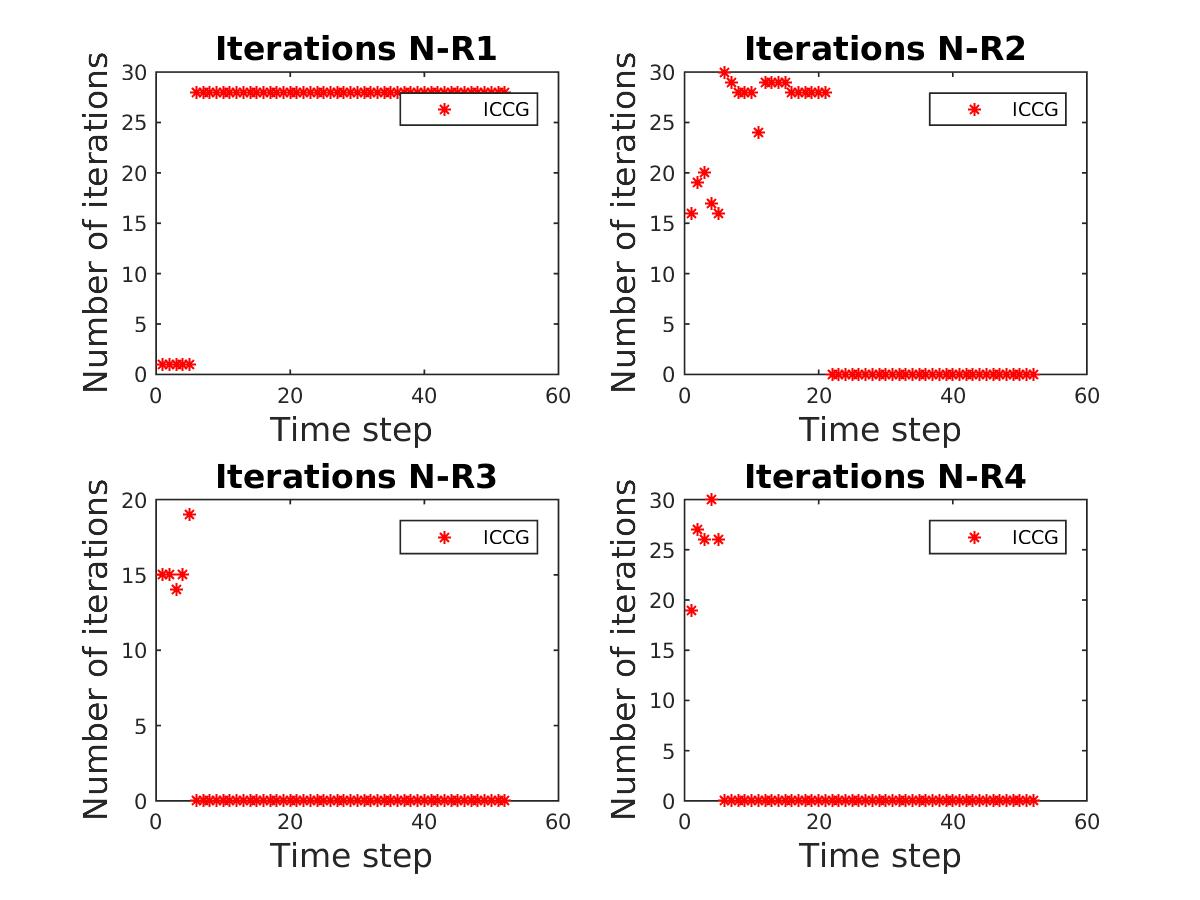
\includegraphics[width=6.5cm,height=6.5cm,keepaspectratio]
{iterations_4NRvw_IC.jpg}
\caption{Number of iterations of the ICCG method for the first four NR iterations.}
\label{fig:vwNR_IC}
\end{minipage}
\end{figure}

\begin{figure}[!h]
\centering
\begin{minipage}{.4\textwidth}
 \centering
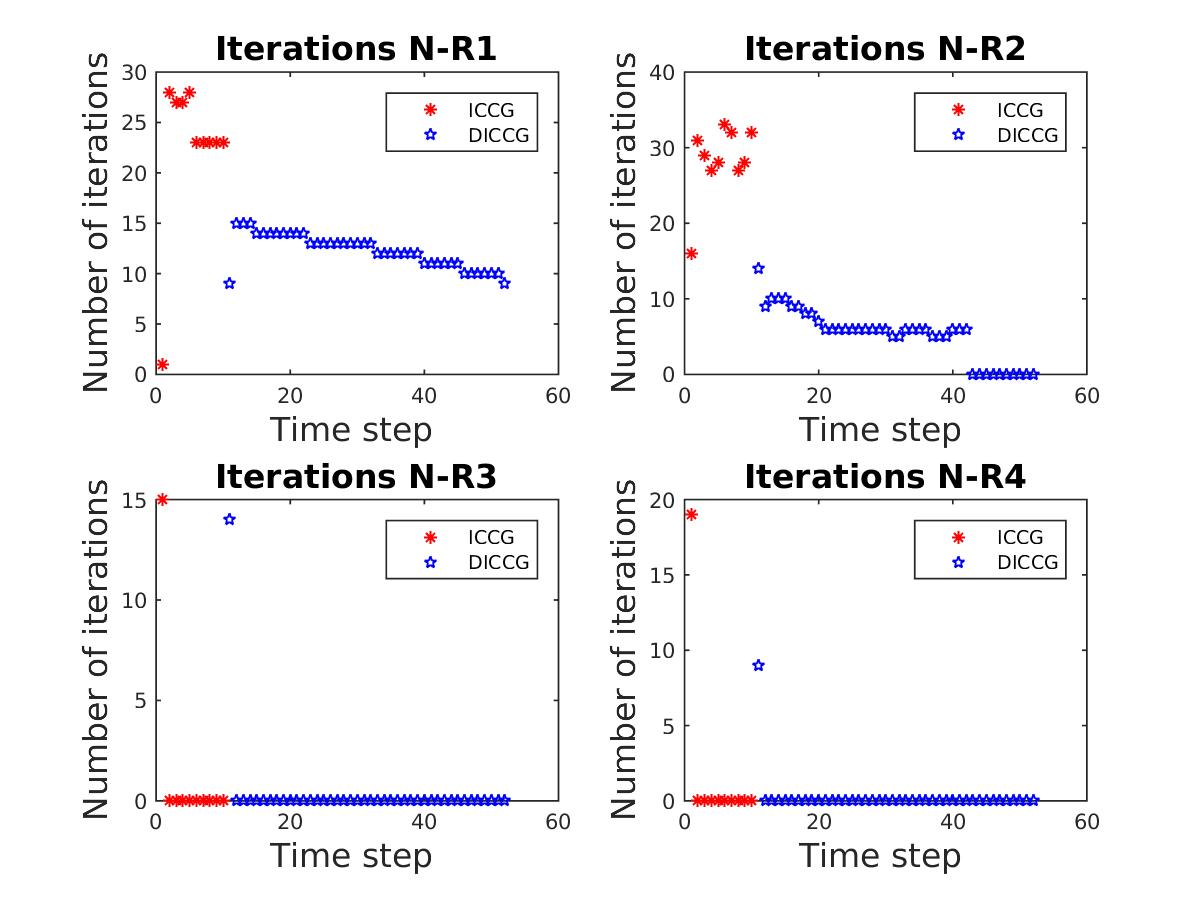
\includegraphics[width=6.5cm,height=6.5cm,keepaspectratio]
{iterations_4NRvw_D10.jpg}
\caption{Number of iterations of the DICCG$_{10}$ method for the first four NR iterations.}
\label{fig:vwNR_D10}
\end{minipage}%
\hspace{15mm}
\begin{minipage}{.4\textwidth}
 \centering
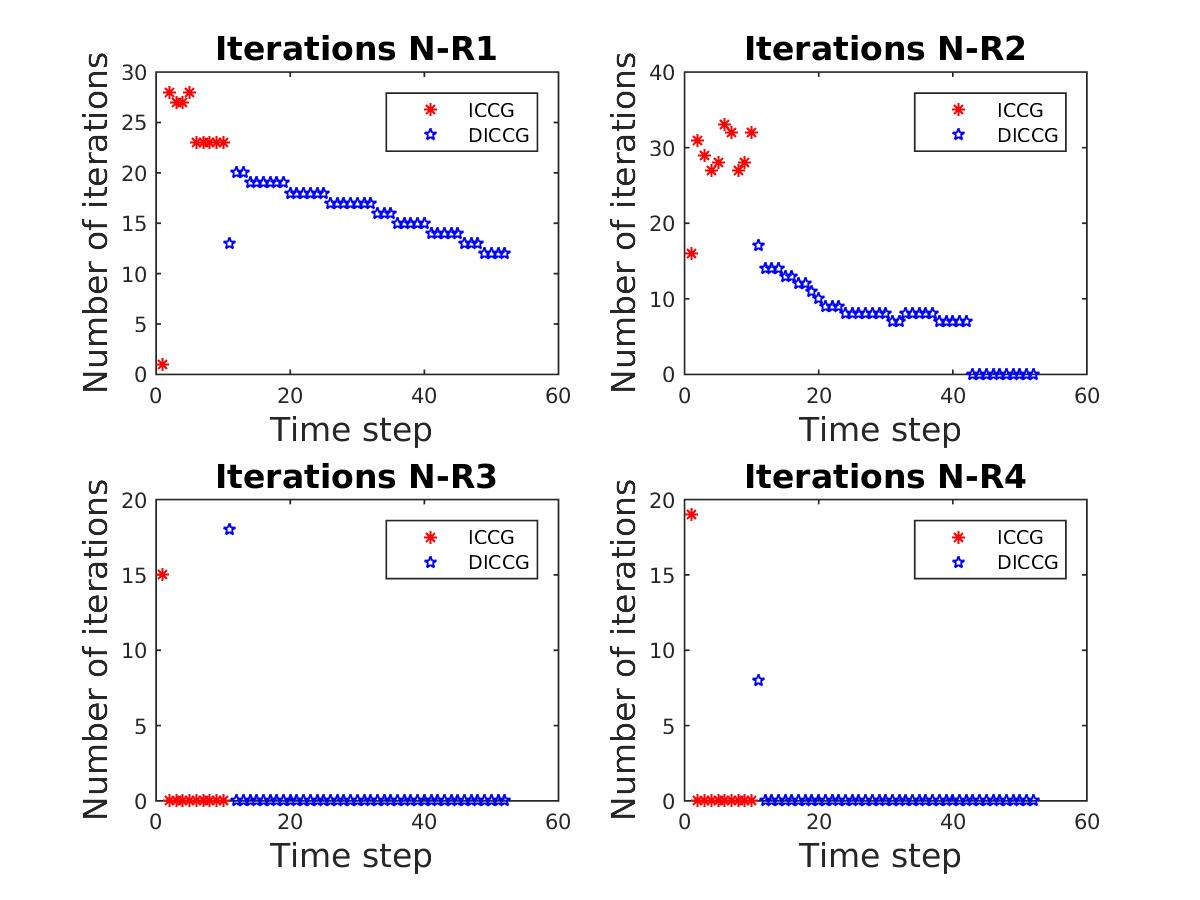
\includegraphics[width=6.5cm,height=6.5cm,keepaspectratio]
{iterations_4NRvw_POD5.jpg}
\caption{Number of iterations of the DICCG$_{POD}$ method for the first four NR iterations.}
\label{fig:vwNR_POD5}
\end{minipage}
\end{figure}
As in the previous case, we observe that the number of iterations for the first and second NR iterations is lower for the deflated methods compared with the ICCG method. However, we observe that the time step when convergence is achieved for the NR cycle is larger for these methods with respect to the ICCG method. We also observe that for the first NR iteration, the reduction is larger for the deflated method with 10 snapshots as deflation vectors.


\newpage
\newpage
\bibliographystyle{unsrt}
\bibliography{research}

\end{document}